\subsection{Software Architecture}

Since the MCU used for this project, in turn uses an ARM Cortex-M processor
core, the software for this project is based on the CMSIS \ref{CMSIS} codebase
supplied from ARM. The Giant Gecko MCU from Silicon Labs is supplied with an API
called emlib \ref{emlib}, which builds upon CMSIS, and can be used to both
initialize and control all attached peripherals. The structure of the code and
programming model is based on the interface with emlib. The code and models
mostly used the emlib API for communicating and controlling the microcontoller.

\begin{figure}[H]
    \centering
    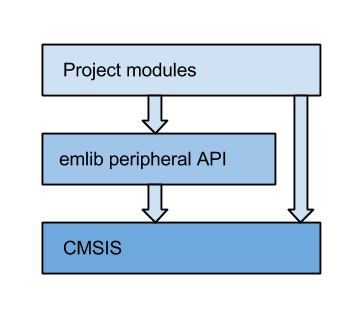
\includegraphics[height=150px]{figures/sw/software-stack.png}
    \caption{The software stack used on the microcontroller}
    \label{fig:software-stack}
\end{figure}


The application code is structured into directories representing each of the
modules or peripherals, whose software was explicity written for this project.
Each directory contains three sub-directories, \textit{inc}, \textit{src} and
\textit{demo}. These sub-directories contain either header files, source files,
or different demos and test programs for each module, respectively. Each module
is typically implemented as a combination of a driver and controller for the
specific peripheral the module is designed for.
